\documentclass[a4paper,11pt]{article}
\usepackage[top=1in, bottom=1in, left=1in, right=1in]{geometry}
% ----- Packages -----
\usepackage{amsmath, amssymb, amsthm} % Advanced math
\usepackage{mathtools} % Extra math tools
\usepackage{physics} % Derivatives, integrals, and more
\usepackage{enumitem} % Better lists
\usepackage{graphicx} % For images if needed
\usepackage[labelformat=empty]{caption}
\usepackage{xcolor} % Colors for emphasis
\usepackage{hyperref} % Clickable links
\usepackage{tcolorbox} % Colored boxes for highlighting key points
\usepackage{multicol}
\usepackage{tabularx}
\usepackage{parcolumns}
\tcbuselibrary{listings,theorems}
\tcbuselibrary{breakable}
\usepackage{centernot}
\usepackage{xcolor}
\usepackage{soul}
\usepackage{ltablex}
% ----- Custom Commands -----
\newcommand{\R}{\mathbb{R}} % Real numbers
\newcommand{\N}{\mathbb{N}} % Natural numbers
\newcommand{\Z}{\mathbb{Z}} % Integers
\newcommand{\Q}{\mathbb{Q}} % Rational numbers
\newcommand{\C}{\mathbb{C}} % Complex numbers

% ----- Theorem Styles -----
\theoremstyle{definition}
\newtheorem{definition}{Definition}

\theoremstyle{plain}
\newtheorem{theorem}{Theorem}
\newtheorem{proposition}{Proposition}
\newtheorem{lemma}{Lemma}
\newtheorem{corollary}{Corollary}

\theoremstyle{remark}
\newtheorem{example}{Example}
\newtheorem{remark}{Remark}

% ----- Title -----
\title{Calculus Notes}
\author{Abror Maksudov}
\date{\today}

\everymath{\displaystyle}

\begin{document}

\maketitle
\tableofcontents

\section{Limits}


% % PRECISE DEFINITION OF A LIMIT


\subsection{Precise Definition of a Limit}

\begin{tcolorbox}
    \textbf{Standard Limit:}  
    \[
    \lim_{x \to a} f(x) = L \quad \text{if} \quad \forall \varepsilon > 0, \, \exists \delta > 0 \text{ such that } 0 < |x - a| < \delta \Rightarrow |f(x) - L| < \varepsilon.
    \]
\end{tcolorbox}


% PRECISE DEFINITION OF ONE-SIDED LIMIT

\subsection{Precise Definition of One-Sided Limit}

\begin{tcolorbox}
\textbf{Right-Hand Limit:}  
\[
\lim_{x \to a^+} f(x) = L \quad \text{if} \quad \forall \varepsilon > 0, \, \exists \delta > 0 \text{ such that } 0 < x - a < \delta \Rightarrow |f(x) - L| < \varepsilon.
\]

\textbf{Left-Hand Limit:}  
\[
\lim_{x \to a^-} f(x) = L \quad \text{if} \quad \forall \varepsilon > 0, \, \exists \delta > 0 \text{ such that } 0 < a - x < \delta \Rightarrow |f(x) - L| < \varepsilon.
\]
\end{tcolorbox}


% PRECISE DEFINITION OF INFINITE LIMIT


\subsection{Precise Definition of Infinite Limit}

\begin{tcolorbox}
\textbf{Infinite Limit:}  
\[
\lim_{x \to a} f(x) = \infty \quad \text{if} \quad \forall M > 0, \, \exists \delta > 0 \text{ such that } 0 < |x - a| < \delta \Rightarrow f(x) > M.
\]
\[
\lim_{x \to a} f(x) = -\infty \quad \text{if} \quad \forall M > 0, \, \exists \delta > 0 \text{ such that } 0 < |x - a| < \delta \Rightarrow f(x) < -M.
\]
\end{tcolorbox}


% PRECISE DEFINITION OF LIMIT AT INFINITY


\subsection{Precise Definition of a Limit at Infinity}

\begin{tcolorbox}
\textbf{Limit at Infinity:}
\[
\lim_{x \to \infty} f(x) = L \quad \text{if} \quad \forall \varepsilon > 0, \, \exists M > 0 \text{ such that } x > M \Rightarrow |f(x) - L| < \varepsilon.
\]
\[
\lim_{x \to -\infty} f(x) = L \quad \text{if} \quad \forall \varepsilon > 0, \, \exists M > 0 \text{ such that } x < -M \Rightarrow |f(x) - L| < \varepsilon.
\]
\end{tcolorbox}


% PRECISE DEFINITION OF INFINITE LIMIT AT INFINITY


\subsection{Precise Definition of Infinite Limit at Infinity}

\begin{tcolorbox}
\textbf{Infinite Limit at Infinity:}  
\[
\lim_{x \to \infty} f(x) = \infty \quad \text{if} \quad \forall M > 0, \, \exists N > 0 \text{ such that } x > N \Rightarrow f(x) > M.
\]
\[
\lim_{x \to \infty} f(x) = -\infty \quad \text{if} \quad \forall M > 0, \, \exists N > 0 \text{ such that } x > N \Rightarrow f(x) < -M.
\]
\[
\lim_{x \to -\infty} f(x) = \infty \quad \text{if} \quad \forall M > 0, \, \exists N > 0 \text{ such that } x < -N \Rightarrow f(x) > M.
\]
\[
\lim_{x \to -\infty} f(x) = -\infty \quad \text{if} \quad \forall M > 0, \, \exists N > 0 \text{ such that } x < -N \Rightarrow f(x) < -M.
\]
\end{tcolorbox}


% LIMIT LAWS


\subsection{Limit Laws}

\begin{tcolorbox}
    Suppose that \(c\) is a constant and the limits \(\displaystyle \lim_{x \to a} f(x)\) and \(\displaystyle \lim_{x \to a} g(x)\) exist. Then
    \begin{enumerate}
        \item \(\displaystyle \lim_{x \to a} c = c\)
        \item \(\displaystyle \lim_{x \to a} x = a\)
        \item \(\displaystyle \lim_{x \to a} [f(x) \pm g(x)] = \lim_{x \to a} f(x) \pm \lim_{x \to a} g(x)\)
        \item \(\displaystyle \lim_{x \to a} [c f(x)] = c \lim_{x \to a} f(x)\)
        \item \(\displaystyle \lim_{x \to a} [f(x) g(x)] = \lim_{x \to a} f(x) \cdot \lim_{x \to a} g(x)\)
        \item \(\displaystyle \lim_{x \to a} \frac{f(x)}{g(x)} = \frac{\displaystyle \lim_{x \to a} f(x)}{\displaystyle \lim_{x \to a} g(x)},\ \text{if } \lim_{x \to a} g(x) \neq 0\)
        \item \(\displaystyle \lim_{x \to a} [f(x)]^n = [\lim_{x \to a} f(x)]^n\)
        \item \(\displaystyle \lim_{x \to a} \sqrt[n]{f(x)} = \sqrt[n]{\lim_{x \to a} f(x)}\)
    \end{enumerate}
\end{tcolorbox}


% RELATIONSHIP BETWEEN THE LIMIT AND ONE-SIDED LIMITS


\subsection{Relationship between the Limit and One-Sided Limits}

\begin{tcolorbox}
    \[\lim_{x \to a} f(x) = L \quad \Leftrightarrow \quad \lim_{x \to a^+} f(x) = \lim_{x \to a^-} f(x) = L.\]
    \[\lim_{x \to a^+} f(x) \neq \lim_{x \to a^-} f(x) \quad \Rightarrow \quad \lim_{x \to a} f(x) \text{ does not exist}.\]
\end{tcolorbox}


% COMPARISON THEOREM


\subsection{Comparison Theorem}

\begin{tcolorbox}
    If \( f(x) \leq g(x) \) when \( x \) is near \( a \), and \(\lim\limits_{x \to a} f(x)\) and \(\lim\limits_{x \to a} g(x)\) exist, then \[\lim\limits_{x \to a} f(x) \leq \lim\limits_{x \to a} g(x).\]
\end{tcolorbox}


% SQUEEZE THEOREM


\subsection{Squeeze Theorem}

\begin{tcolorbox}
    If \( f(x) \leq g(x) \leq h(x) \) when \( x \) is near \( a \), and
    \[ \lim\limits_{x \to a} f(x) = \lim\limits_{x \to a} h(x) = L \] then
    \[\lim\limits_{x \to a} g(x) = L.\]
\end{tcolorbox}


% CONTINUITY


\subsection{Continuity}

\begin{tcolorbox}
    A function \( f(x) \) is \textbf{continuous at} \( x = a \) if and only if it satisfies \textbf{all} the following:
    \[
    \begin{aligned}
        &\text{(1)} \quad f(a) \text{ exists} \\  
        &\text{(2)} \quad \lim\limits_{x \to a} f(x) \text{ exists} \\  
        &\text{(3)} \quad \lim\limits_{x \to a} f(x) = f(a)  
    \end{aligned}
    \]
    Otherwise, \( f(x) \) is discontinuous at \( x = a \).
\end{tcolorbox}


% PROPERTIES OF CONTINUOUS FUNCTIONS


\subsection{Properties of Continuous Functions}


\begin{tcolorbox}
    If \( f(x) \) and \( g(x) \) are continuous at \( x = a \) and \( c \) is a constant, then the following functions are also continuous at \( x = a \):  
    \begin{enumerate}
        \begin{multicols}{3}
            \item \(f + g\)
            \item \(f - g\)
            \item \(cf\)
        \end{multicols}
        \begin{multicols}{3}
            \item \(fg\)
            \item \(\displaystyle \frac{f}{g} \quad \) if \( g(a) \neq 0\)
        \end{multicols}
    \end{enumerate}
\end{tcolorbox}



% TYPES OF DISCONTINUITY


\subsection{Types of Discontinuity}

\begin{figure}[htbp]
    \centering
    \includegraphics[width=\textwidth]{4-types-of-discontinuity.png} 
    \caption{Source: calcworkshop.com}
    \label{fig:discontinuity}
\end{figure}


% LIMITS OF CONTINUOUS FUNCTIONS

\subsection{Limits of Continuous Functions}

\begin{tcolorbox}
    If \( f(x) \) is continuous at \( b \) and \( \displaystyle \lim_{x \to a} g(x) = b \),  then
    \[ \lim_{x \to a} f(g(x)) = f( \lim_{x \to a} g(x) ) = f(b). \]
    \tcblower
    If \( g \) is continuous at \( a \) and \( f \) is continuous at \( g(a) \), then the composite \( f \circ g \) is continuous at \( a \).
\end{tcolorbox}


% INTERMEDIATE VALUE THEOREM


\subsection{Intermediate Value Theorem}

\begin{tcolorbox}
    If \( f \) is continuous on a closed interval \( [a, b] \), then for any \( N \) between \( f(a) \) and \( f(b) \),  
    \[
    \exists \; c \in [a,b] \text{ such that } f(c) = N
    \]
\end{tcolorbox}


% ASYMPTOTES


\subsection{Asymptotes}

\begin{tcolorbox}[breakable]
    \textbf{Vertical Asymptote:} 
    \( x = a \) is a vertical asymptote if  
    \[
    \lim\limits_{x \to a^{\pm}} f(x) = \pm\infty.
    \]
    
    \textbf{Horizontal Asymptote:}
    \( y = L \) is a horizontal asymptote if  
    \[
    \lim\limits_{x \to \pm\infty} f(x) = L.
    \]
    For \( \displaystyle f(x) = \frac{P(x)}{Q(x)} \), compare degrees of \( P \) and \( Q \):  
    \[
    \begin{aligned}
        &\deg P < \deg Q \quad \Rightarrow \quad y = 0. \\  
        &\deg P = \deg Q \quad \Rightarrow \quad y = \frac{\text{leading coef. of } P}{\text{leading coef. of } Q}. \\  
        &\deg P > \deg Q \quad \Rightarrow \quad \text{no horizontal asymptote}.
    \end{aligned}
    \]

    \textbf{Oblique Asymptote:}
    \( y = mx + b \) is an oblique asymptote if  
    \[
    \lim\limits_{x \to \pm\infty} \big( f(x) - (mx + b) \big) = 0.
    \]
    For a rational function \( \displaystyle f(x) = \frac{P(x)}{Q(x)} \), if \( \deg P = \deg Q + 1 \), then \( f(x) \) has an oblique asymptote.  
    Find it by polynomial long division:  
    \[
    f(x) = D(x) + \frac{R(x)}{Q(x)}, \quad \text{as } x \to \pm\infty, \quad f(x) \approx D(x).
    \]
    
    \newpage
    
    \textbf{Curvilinear Asymptote:}
    \( y = g(x) \) is a curvilinear asymptote if
    \[
    \lim\limits_{x \to \pm\infty} \big( f(x) - g(x) \big) = 0,
    \]
    where \( g(x) \) is any non-linear function.
\end{tcolorbox}


% COMMON LIMITS


\subsection{Common Limits}

\begin{tcolorbox}
    Assume $a > 0$ in the following.
    
    \begin{multicols}{2}
        \begin{enumerate}
            \item \( \lim\limits_{x \to 0} \frac{\sin ax}{bx} = \frac{a}{b} \)
            \item \( \lim\limits_{x \to 0} \frac{\tan ax}{bx} = \frac{a}{b} \)
            \item \( \lim\limits_{x \to 0} \frac{1 - \cos x}{x} = 0 \)
            \item \( \lim\limits_{x \to 0} \frac{1 - \cos x}{x^2} = \frac{1}{2} \)
            \item \( \lim\limits_{x \to 0} \frac{e^{ax} - 1}{x} = a \)
            \item \( \lim\limits_{x \to 0} \frac{a^x - 1}{x} = \ln a \)
            \item \( \lim\limits_{x \to 0} \left(1 + \frac{k}{x}\right)^{mx} = e^{mk} \)
            \item \( \lim\limits_{x \to 0} \frac{\ln(1 + x)}{x} = 1 \)
            \item \( \lim\limits_{x \to 0} \frac{\log_a(1 + x)}{x} = \log_a e \)
            \item \( \lim\limits_{x \to 0^+} x^x = 1 \)
            \item \( \lim\limits_{x \to 0^+} x^a \ln x = 0 \)
            \item \( \lim\limits_{x \to +\infty} x^{-a} \ln x = 0 \)
        \end{enumerate}
    \end{multicols}
        
\end{tcolorbox}


% --------------------------------------------------


\section{Derivatives}


% DERIVATIVE AT A POINT


\subsection{Derivative at a Point}

\begin{tcolorbox}
    The \textbf{derivative} of \( f(x) \) at \( x = a \) is the \textbf{instantaneous rate of change} at that point:
    \[
    f'(a) = \left. \frac{df}{dx} \right|_{x=a} =\lim\limits_{h \to 0} \frac{f(a + h) - f(a)}{h} = \lim\limits_{x \to a} \frac{f(x) - f(a)}{x - a}.
    \]
\end{tcolorbox}


% DERIVATIVE AT A POINT


\subsection{Derivative as a Function}

\begin{tcolorbox}
    The derivative of a function \( f(x) \) at a point \( x \) is defined as the limit
    \[
    f'(x) = \lim_{\Delta x \to 0} \frac{f(x + \Delta x) - f(x)}{\Delta x}.
    \]
\end{tcolorbox}


% DIFFERENTIABILITY


\subsection{Differentiability}

\begin{tcolorbox}
    A function \( f(x) \) is \textbf{differentiable} at \( x = a \) if its derivative \( f'(x) \) exists. That is:  
    \[
    f(x) \text{ is differentiable at } x = a \iff \text{ The limit } \lim\limits_{h \to 0} \frac{f(a+h) - f(a)}{h} \text{ exists.}
    \]
\end{tcolorbox}


% DIFFERENTIABILITY IMPLIES CONTINUITY


\subsection{Differentiability Implies Continuity}

\begin{tcolorbox}
    If \( f(x) \) is differentiable at \( x = a \), then it is continuous at \( x = a: \)
    \[
    f \text{ differentiable at } a \implies f \text{ continuous at } a.
    \]
    However, the converse is false:
    \[
    f \text{ continuous at } a \centernot\implies f \text{ differentiable at } a.
    \]
\end{tcolorbox}


% PROPERTIES OF DERIVATIVES


\subsection{Properties of Derivatives}

\begin{tcolorbox}
    Let $f(x)$ and $g(x)$ be differentiable functions. Then the following rules hold:
    \[
    \begin{aligned}
        &\text{(1)} \quad \frac{d}{dx}(c) = 0. \\[8pt]  
        &\text{(2)} \quad \frac{d}{dx}(x^n) = nx^{n-1}. \\[8pt]
        &\text{(3)} \quad \frac{d}{dx}[cf(x)] = c[\frac{d}{dx}f(x)]. \\[8pt]
        &\text{(4)} \quad \frac{d}{dx}[f(x) \pm g(x)] = \frac{d}{dx}f(x) \pm \frac{d}{dx}g(x). \\[8pt]
        &\text{(5)} \quad \frac{d}{dx}[f(x)g(x)] = f'(x)g(x) + f(x)g'(x). \\[8pt]
        &\text{(6)} \quad \frac{d}{dx}[\frac{f(x)}{g(x)}] = \frac{f'(x)g(x) - f(x)g'(x)}{g(x)^2}. \\[8pt]
        &\text{(7)} \quad \frac{d}{dx}[f(g(x))] = f'(g(x))g'(x). \\[8pt]
    \end{aligned}
    \]
\end{tcolorbox}


% TABLE OF DERIVATIVES


\subsection{Table of Derivatives}

\begin{tcolorbox}
    \begin{tabularx}{\textwidth}{X|X|X}
         $(\sin x)' = \cos x$ & 
         $(\arcsin x)' = \frac{1}{\sqrt{1-x^2}}$ & 
         $(e^x)' = e^x$ \\[10pt]
         
         $(\cos x)' = -\sin x$ & 
         $(\arccos x)' = -\frac{1}{\sqrt{1-x^2}}$ & 
         $(a^x)' = a^x\ln{a}$ \\[10pt]
         
         $(\tan x)' = \sec^2 x$ & 
         $(\arctan x)' = \frac{1}{1+x^2}$ & 
         $(\log_a{x})' = \frac{1}{x\ln{a}}$ \\[10pt]
         
         $(\cot x)' = -\csc^2 x$ & 
         $(\arccot x)' = -\frac{1}{1+x^2}$ & 
         $(\ln{x})' = \frac{1}{x}$ \\[10pt]
         
         $(\sec x)' = \sec x \tan x $ & 
         $(\arcsec x)' = \frac{1}{x\sqrt{x^2-1}}$ & 
         $(\left| x \right|)' = \frac{x}{|x|}$ \\[10pt]
         
         $(\csc x)' = -\csc x \cot x $ & 
         $(\arccsc x)' = -\frac{1}{x\sqrt{x^2-1}}$ & 
         $(x^x)' = x^x(1+\ln{x})$ \\[10pt]
    \end{tabularx}
\end{tcolorbox}



% ABSOLUTE AND LOCAL EXTREMA


\subsection{Absolute and Local Extrema}

\begin{tcolorbox}
    Let $f$ be defined on a domain $D$, and let $c \in D$.
    \begin{itemize}
        \item \textbf{Absolute Maximum:} $f(c)$ is an absolute maximum if $f(c) \geq f(x),\ \forall x \in D.$
        \item \textbf{Absolute Minimum:} $f(c)$ is an absolute minimum if $f(c) \leq f(x),\ \forall x \in D.$
        \item \textbf{Local Maximum:} $f(c)$ is a local maximum if $\exists \delta > 0$ such that $f(c) \geq f(x),\\ \quad \forall x \in (c - \delta, c + \delta).$
        \item \textbf{Local Minimum:} $f(c)$ is a local minimum if $\exists \delta > 0$ such that $f(c) \leq f(x),\\ \quad \forall x \in (c - \delta, c + \delta).$
    \end{itemize}
\end{tcolorbox}


% EXTREME VALUE THEOREM


\subsection{Extreme Value Theorem}

\begin{tcolorbox}
    If $f$ is continuous on a closed interval $[a,b]$, then $f$ attains an absolute maximum and an absolute minimum on $[a,b]$:
    \[
    \exists c,d \in [a,b] \text{ such that } f(c) \leq f(x) \leq f(d),\quad \forall x \in [a,b].
    \]
\end{tcolorbox}


% CRITICAL AND STATIONARY POINTS


\subsection{Critical and Stationary Points}

\begin{tcolorbox}
    Let $f$ be defined on an interval $I$ and $c \in I.$
    \begin{itemize}
        \item \textbf{Critical Point:} $c$ is a critical point of $f$ if either
        \begin{enumerate}
            \item $f'(c) = 0$, or
            \item $f'(c)$ does not exist
        \end{enumerate}
        \item \textbf{Stationary Point:} $c$ is a stationary point of $f$ if $f'(c) = 0.$        
    \end{itemize}
    Note: \textit{Every stationary point is a critical point, but not conversely.}
\end{tcolorbox}


% ROLLE'S THEOREM


\subsection{Rolle's Theorem}

\begin{tcolorbox}
    Let $f$ satisfy all conditions:
    \begin{enumerate}
        \item $f$ is continuous on $[a,b]$.
        \item $f$ is differentiable on $(a,b)$.
        \item $f(a) = f(b)$.
    \end{enumerate}
    Then, there exists at least one $c \in (a,b)$ such that $f'(c) = 0$.
\end{tcolorbox}


% MEAN VALUE THEOREM


\subsection{Mean Value Theorem}

\begin{tcolorbox}
    Let $f$ satisfy all conditions:
    \begin{enumerate}
        \item $f$ is continuous on $[a,b]$.
        \item $f$ is differentiable on $(a,b)$.
    \end{enumerate}
    Then, there exists at least one $c \in (a,b)$ such that:
    \[
    f'(c) = \frac{f(b) - f(a)}{b-a}.
    \]
    Note: Rolle's Theorem is a special case of the Mean Value Theorem where $f(a) = f(b)$.
\end{tcolorbox}


% INCREASING/DECREASING TEST


\subsection{Increasing/Decreasing Test}

\begin{tcolorbox}
    Let $f$ be differentiable on an interval $I$. Then, for all $x \in I$:
    \begin{enumerate}
        \item If $f'(x) > 0$, then $f$ is strictly increasing on $I$.
        \item If $f'(x) < 0$, then $f$ is strictly decreasing on $I$.
        \item If $f'(x) = 0$, then $f$ is constant on $I$.
    \end{enumerate}
\end{tcolorbox}


% FIRST DERIVATIVE TEST


\subsection{First Derivative Test}

\begin{tcolorbox}
    Let $c$ be a critical point of a differentiable function $f(x)$, meaning $f'(c)=0$ or $f'(c)$ does not exist. Then:
    \begin{enumerate}
        \item If $f'(x)$ changes from positive to negative at $x=c$, then $f(c)$ is a \textbf{local maximum}.
        \item If $f'(x)$ changes from negative to positive at $x=c$, then $f(c)$ is a \textbf{local minimum}.
        \item If $f'(x)$ does not change sign at $x=c$, then $f(c)$ is \textbf{neither} a local maximum nor a local minimum.
    \end{enumerate}
\end{tcolorbox}


% CONCAVITY AND INFLECTION POINTS


\subsection{Concavity and Inflection Points}

\begin{tcolorbox}
    \[\text{Concave up} \iff \text{Curve \textbf{lies above} all of its \textbf{tangent lines}}.\]
    \[\text{Concave down} \iff \text{Curve \textbf{lies below} all of its \textbf{tangent lines}}.\]
    \[\text{Inflection point} \iff \text{Point where \textbf{concavity changes}}.\]
\end{tcolorbox}


% CONCAVITY TEST


\subsection{Concavity Test}

\begin{tcolorbox}
    Let $f(x)$ be twice differentiable on interval $I$. Then:
    \begin{itemize}
        \item If $f''(x) > 0, \quad \forall x \in I \implies f(x)$ is \textbf{concave up} on $I$.
        \item If $f''(x) < 0, \quad \forall x \in I \implies f(x)$ is \textbf{concave down} on $I$.
    \end{itemize}
\end{tcolorbox}


% SECOND DERIVATIVE TEST


\subsection{Second Derivative Test}

\begin{tcolorbox}
    Let $c$ be a critical point of $f$ where $f(c)=0$. If $f''(c)$ exists, then:
    \begin{enumerate}
        \item If $f''(c) > 0$, $f(x)$ is \textbf{concave up} at $c$, so $f(c)$ is a \textbf{local minimum}.
        \[ \text{Local Maximum at $c$} \iff f'(c) = 0 \text{ and } f''(c) < 0 \]
        \item If $f''(c) < 0$, $f(x)$ is \textbf{concave down} at $c$, so $f(c)$ is a \textbf{local maximum}.
        \[ \text{Local Minimum at $c$} \iff f'(c) = 0 \text{ and } f''(c) > 0 \]
        \item If $f''(c) = 0$ or \textbf{does not exist}, the test is \textbf{inconclusive}---use the First Derivative Test instead.
    \end{enumerate}
\end{tcolorbox}


% L'HÔPITAL'S RULE


\subsection{L'Hôpital's Rule}

\begin{tcolorbox}
    Let $f(x)$ and $g(x)$ be differentiable on an open interval containing $a$ (except possibly at $a$). If 
    \[ 
    \lim_{x \to a} f(x) = \lim_{x \to a} g(x) = 0 \text{ or } \lim_{x \to a} f(x) = \lim_{x \to a} g(x) = \pm \infty 
    \]
    then
    \[
    \lim_{x \to a} \frac{f(x)}{g(x)} = \lim_{x \to a} \frac{f'(x)}{g'(x)}.
    \]
\end{tcolorbox}


% INDETERMINATE FORMS


\subsection{Indeterminate Forms}

\begin{tcolorbox}
    The following symbols are “indeterminate”:
    \begin{center}
        \begin{minipage}{10cm}
            $\frac{0}{0}$ \hspace*{\fill} $\frac{\infty}{\infty}$ \hspace*{\fill} 
            $0 \cdot \infty$ \hspace*{\fill} $\infty - \infty$ \hspace*{\fill} 
            $1^\infty$ \hspace*{\fill} $0^\infty$ \hspace*{\fill} $\infty ^ 0$
        \end{minipage}
    \end{center}
    \textit{Warning}: The following symbols are \textit{not} indeterminate:
    \begin{center}
        \begin{minipage}{10cm}
            $\frac{1}{0}$ \hspace*{\fill} $\frac{\infty}{0}$ \hspace*{\fill} 
            $\frac{1}{\infty}$ \hspace*{\fill} $1 \cdot \infty$ \hspace*{\fill} 
            $\infty + \infty$ \hspace*{\fill} $1 + \infty$ \hspace*{\fill} $0 ^ \infty$
        \end{minipage}
    \end{center}
\end{tcolorbox}


% --------------------------------------------------


\section{Integrals}

% ANTIDERIVATIVES


\subsection{Antiderivatives}

\begin{tcolorbox}
    A function $F(x)$ is an \textbf{antiderivative} (or primitive function) of $f(x)$ on an interval $I$ if:
    \[ F'(x) = f(x), \quad \forall x \in I. \]
\end{tcolorbox}


% INDEFINITE INTEGRALS


\subsection{Indefinite Integrals}

\begin{tcolorbox}
    The \textbf{indefinite integral} (or general antiderivative) of a function $f(x)$ is the family of all its antiderivatives:
    \[ \int f(x) dx = F(x) + C \]
    where $F(x)$ is any antiderivative of $f(x)$ and $C$ is an arbitrary constant.
\end{tcolorbox}


% RIEMANN SUM

\subsection{Riemann Sum}

\begin{tcolorbox}
    Let $f(x)$ be a function defined on a closed interval $[a,b]$ , and let the interval be partitioned into $n$ subintervals by inserting $n-1$ points $x_1, x_2, \dots, x_{n-1}$ such that:
    \[
    a = x_0 < x_1 < x_2 < \dots < x_{n} = b
    \]
    where the subintervals $[x_{i-1}, x_i]$ have length $\Delta x_i = x_i - x_{i-1}$. For each subinterval $[x_{i-1}, x_i]$, let $x_i^*$  be an \textbf{arbitrary sample point} within the interval. Then, a \textbf{Riemann sum}, which \textbf{approximates} the area under the curve $f(x)$ over $[a,b]$, is defined as:
    \[
    S_n = \sum_{i=1}^n f(x_i^*) \Delta x_i, \quad x_i^* \in [x_{i-1}, x_i].
    \]
\end{tcolorbox}


% PARTITIONS OF AN INTERVAL

\subsection{Partitions of an Interval}

\begin{figure}[htbp]
    \centering
    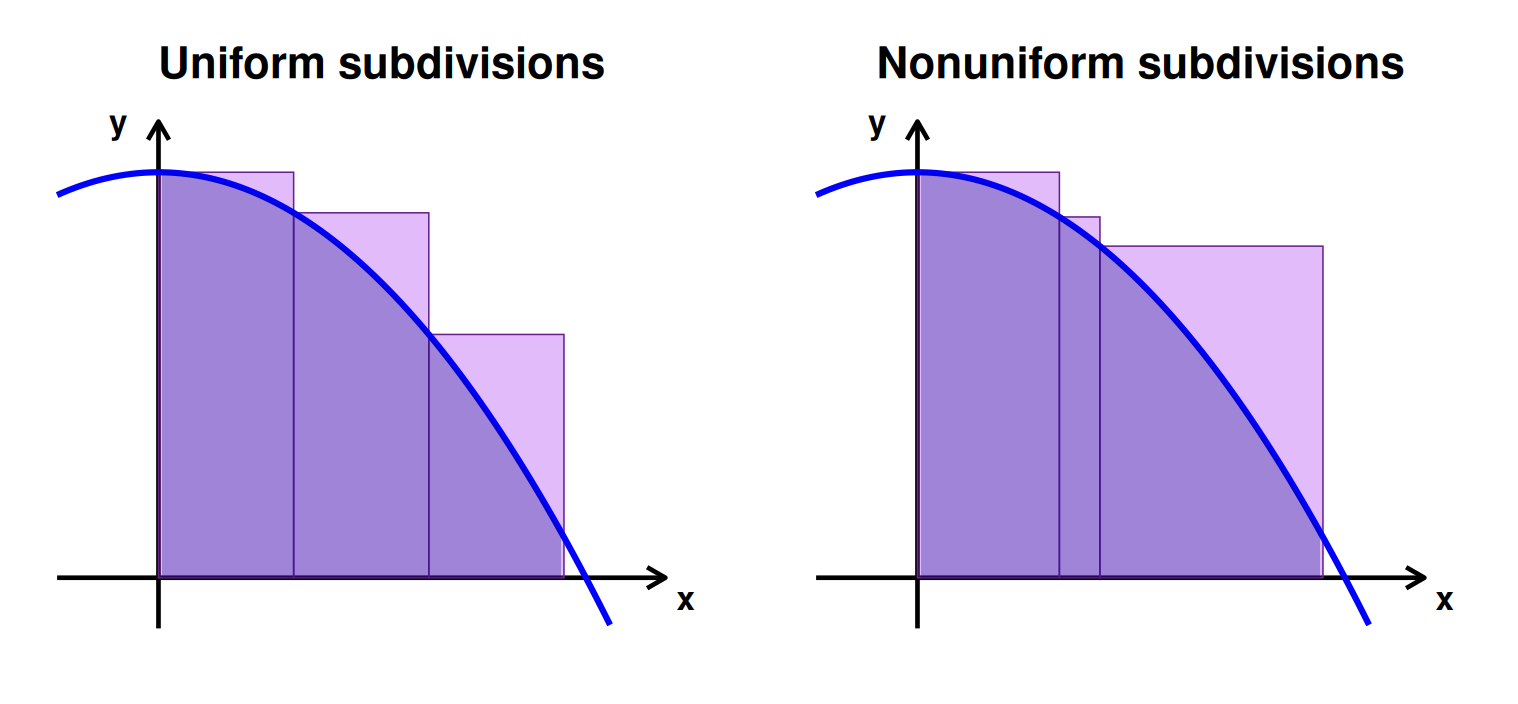
\includegraphics[width=\textwidth]{types-of-partitions.png} 
    \caption{Comparison of uniform and non-uniform partitions of an interval (generated using R).}
    \label{fig:discontinuity}
\end{figure}

\begin{tcolorbox}[breakable]
    A partition of $[a, b]$ divides it into $n$ subintervals:
    \[
    P = \{ a = x_0 < x_1 < x_2 < \dots < x_n = b \}
    \]
    Each subinterval has width:
    \[
    \Delta x_i = x_i - x_{i-1}.
    \]
    \begin{itemize}
        \item \textbf{Uniform Partition:} All subintervals have the same width:
        \[
        \Delta x_i = \Delta x = \frac{b-a}{n}, \quad \forall i.
        \]
        \item \textbf{Non-Uniform Partition:}  Subintervals have different widths, and \( \Delta x_i \) varies for each \( i \).
    \end{itemize}
\end{tcolorbox}


% TYPES OF RIEMANN SUMS

\subsection{Types of Riemann Sums}

\begin{tcolorbox}[breakable]
    The type of Riemann sum depends on how the sample points $x_i^*$ are chosen within each subinterval $[x_{i-1}, x_i]$.
    \begin{enumerate}
        \item \textbf{Arbitrary-Point Rule:} $x_i^* \in [x_{i-1}, x_i] \rightarrow$ \textbf{General Riemann Sum}
        \[
        S_n = \sum_{i=1}^{n} f(x_i^*) \Delta x_i, \quad \Delta x_i = x_i - x_{i-1}.
        \]
        \textbf{Uniform Partition:} If all subintervals have equal width $\Delta x = \frac{b-a}{n}$, then \\ $x_i^* \in [x_{i-1}, x_i] = [a + (i - 1) \Delta x, a + i \Delta x]$ or $x_i^* = a + (i - 1 + c) \Delta x$, where $c \in [0,1]$ determines its position within the subinterval:
        \[
        S_n = \sum_{i=1}^{n} f(a + (i - 1 + c) \Delta x) \Delta x = \sum_{i=1}^{n} f(a + (i - 1 + c) \frac{(b - a)}{n}) \frac{b - a}{n}.
        \]
        $\bullet$ Uses arbitrary sample points $x_i^*$.
    
        \item \textbf{Left Rule:} $x_i^* = x_{i-1}\rightarrow$ \textbf{Left Riemann Sum}
        \[
        S_{\text{left}} = \sum_{i=1}^n f(x_{i-1}) \Delta x_i.
        \]
        \textbf{Uniform Partition:} $c = 0$
        \[
        S_{\text{left}} = \sum_{i=1}^n f(a + (i - 1) \Delta x) \Delta x.
        \]
        $\bullet$ Underestimates for increasing functions, overestimates for decreasing functions.
        
        \item \textbf{Right Rule:} $x_i^* = x_i\rightarrow$ \textbf{Right Riemann Sum}
        \[
        S_{\text{right}} = \sum_{i=1}^n f(x_i) \Delta x_i    
        \]
        \textbf{Uniform Partition:} $c = 1$
        \[
        S_{\text{right}} = \sum_{i=1}^n f(a + i \Delta x) \Delta x.
        \]
        $\bullet$ Overestimates for increasing functions, underestimates for decreasing functions.
        
        \item \textbf{Midpoint Rule:} $x_i^* = \frac{x_{i-1} + x_i}{2} \rightarrow$ \textbf{Midpoint Riemann Sum}
        \[
        S_{\text{mid}} = \sum_{i=1}^n f\left( \frac{x_{i-1} + x_i}{2} \right) \Delta x_i.
        \]
        \textbf{Uniform Partition:} $c = \frac{1}{2}$
        \[
        S_{\text{mid}} = \sum_{i=1}^n f(a + (i - \frac{1}{2}) \Delta x) \Delta x.
        \]
        $\bullet$ Tends to give better approximations than left or right sums.
        
        \item \textbf{Upper Rule:} $x_i^* = \arg\sup\limits_{x \in [x_{i-1}, x_i]} f(x) \rightarrow$ \textbf{Upper Riemann Sum} (or \textbf{Upper Darboux Sum})
        \[
        S_{\text{upper}} = \sum_{i=1}^n \sup\limits_{x \in [x_{i-1}, x_i]} f(x) \Delta x_i.
        \]
        $\bullet$ Always \textbf{overestimates} the integral.

        \pagebreak
        
        \item \textbf{Lower Rule:} $x_i^* = \arg\inf\limits_{x \in [x_{i-1}, x_i]} f(x) \rightarrow$ \textbf{Lower Riemann Sum} (or \textbf{Lower Darboux Sum})
        \[
        S_{\text{lower}} = \sum_{i=1}^n \inf\limits_{x \in [x_{i-1}, x_i]} f(x) \Delta x_i.
        \]
        $\bullet$ Always \textbf{underestimates} the integral.
    \end{enumerate}
\end{tcolorbox}


% DEFINITE INTEGRAL


\subsection{Definite Integral}

\begin{tcolorbox}
    The \textbf{definite integral} of a function $f(x)$ over the interval $[a,b]$ is defined as the limit of a Riemann sum:
    \[
    \int_{a}^{b} f(x) \, dx = \lim_{n \to \infty} \sum_{i=1}^n f(x_i^*) \Delta x_i
    \]
    where:
    \begin{itemize}
        \item $[a,b]$ is divided into $n$ subintervals.
        \item $\Delta x_i = x_i - x_{i-1}$ is the width of the $i$-th subinterval.
        \item $x_i^*$ is any sample point in the $i$-th subinterval.
    \end{itemize}
\end{tcolorbox}
\pagebreak


% PROPERTIES OF DEFINITE INTEGRALS


\subsection{Properties of Definite Integrals}

\begin{tcolorbox}[breakable]
    Let $f(x)$ and $g(x)$ be integrable functions on $[a,b]$ and $c$ be a constant. Then:
    \[
    \begin{aligned}
        &\text{(1)} \quad \int_{a}^{b}c \, dx = c(b-a). \\[8pt]
        &\text{(2)} \quad \int_{a}^{a}f(x) \, dx = 0. \\[8pt]
        &\text{(3)} \quad \int_{b}^{a}f(x) \, dx = -\int_{a}^{b}f(x) \, dx. \\[8pt]
        &\text{(4)} \quad \int_{a}^{b}cf(x) \, dx = c \int_{a}^{b}f(x) \, dx. \\[8pt]
        &\text{(5)} \quad \int_{a}^{b}\left[f(x) \pm g(x)\right] \, dx = \int_{a}^{b}f(x) \, dx \pm \int_{a}^{b}g(x) \, dx. \\[8pt]
        &\text{(6)} \quad \int_{a}^{b}f(x) \, dx = \int_{a}^{c}f(x) \, dx + \int_{c}^{b}f(x) \, dx. \\[8pt]
        &\text{(7)} \quad \int_{a}^{b}f(x) \, dx \leq \int_{a}^{b}g(x) \, dx \quad \text{ if } f(x) \leq g(x) \text{ on } [a,b]. \\[8pt]
        &\text{(8)} \quad \left| \int_{a}^{b}f(x) \, dx \right| \leq \int_{a}^{b} \left|f(x)\right| \, dx. \\[8pt]
        &\text{(9)} \quad m(b-a) \leq \int_{a}^{b}f(x) \, dx \leq M(b-a) \quad \text{ if } m \leq f(x) \leq M \text{ on } [a,b]. \\[8pt]
    \end{aligned}
    \]
\end{tcolorbox}


% NET AND TOTAL AREA


\subsection{Net and Total Area}

\begin{tcolorbox}
    Let $f(x)$ be integrable on $[a,b]$. Define:
    \begin{itemize}
        \item $A_1$ = area of region where $f(x) > 0$ (area above $x$-axis).
        \item $A_2$ = area of region where $f(x) < 0$ (area below $x$-axis).
    \end{itemize}
    Then:
    \begin{itemize}
        \item \textbf{Net Area:}
        \[
        \int_{a}^{b} f(x) \, dx = A_1 - A_2.
        \]
        \item \textbf{Total Area:}
        \[
        \int_{a}^{b} \left| f(x) \right| \, dx = A_1 + A_2.
        \]
    \end{itemize}
\end{tcolorbox}


% MEAN VALUE THEOREM FOR INTEGRALS


\subsection{Mean Value Theorem for Integrals}

\begin{tcolorbox}
    Let $f$ be continuous on [a,b]. Then:
    \[
    \exists c \in (a,b) \text{ such that } \frac{1}{b - a} \int_{a}^{b} f(x) \, dx = f(c)
    \]
    The expression on the left is the \textbf{average value} of the function $f(x)$ on the interval $[a, b]$.
\end{tcolorbox}


% FUNDAMENTAL THEOREM OF CALCULUS. PART 1


\subsection{Fundamental Theorem of Calculus. Part 1}

\begin{tcolorbox}
    Let $f$ be a continuous on $[a, b]$. Define the function
    \[
    F(x) = \int_{a}^{x} f(t) \, dt.
    \]
    Then:
    \[
    F'(x) = \frac{d}{dx} \left[ \int_{a}^{x} f(t) \, dt \right] = f(x), \quad \forall x \in (a,b).
    \]
\end{tcolorbox}


% FUNDAMENTAL THEOREM OF CALCULUS. PART 2


\subsection{Fundamental Theorem of Calculus. Part 2}

\begin{tcolorbox}
    If $f$ is continuous on $[a,b]$ and $F'(x) = f(x)$, then
    \[
    \int_{a}^{b} f(x) \, dx = F(b) - F(a) =  F(x) \bigg]_{a}^{b} = F(x) \bigg|_{a}^{b}.
    \]
\end{tcolorbox}


% TABLE OF INDEFINITE INTEGRALS


\subsection{Table of Indefinite Integrals}

\begin{tcolorbox}[breakable]
    \keepXColumns
    \begin{tabularx}{\textwidth}{X|X}
        $\int a \, dx = ax + C$ &  
        $\int \log_a x \, dx = \frac{x}{\ln{a}} (\ln{x} - 1) + C$ \\[12pt] 

        $\int x^n \, dx = \frac{x^{n+1}}{n+1} + C,\quad n \neq -1$ &
        $\int (ax+b)^n \, dx = \frac{(ax+b)^{n+1}}{a(n+1)} + C$ \\[12pt]
        
        $\int x^{-1} \, dx = \int \frac{1}{x} \, dx = \ln{|x|} + C$ &
        $\int \frac{c}{ax+b} \, dx = \frac{c}{a} \ln{|ax+b|} + C$ \\[12pt] 
        
        $\int e^{ax} \, dx = \frac{1}{a} e^{ax} + C$ &
        $\int a^x \, dx = \frac{a^x}{\ln{a}} + C,\quad a > 0,\; a \neq 1$ \\[12pt]
              
        $\int \sin{x} \, dx = - \cos{x} + C$ &
        $\int \tan{x} \, dx = \ln{|\sec{x}|} = - \ln{|\cos{x}|} + C$ \\[12pt]
              
        $\int \cos{x} \, dx = \sin{x} + C$ &
        $\int \cot{x} \, dx = -\ln{|\csc{x}|} = \ln{|\sin{x}|} + C$ \\[12pt]
        
        $\int \sec{x} \, dx = \ln{|\sec{x} + \tan{x}|} + C$ &
        $\int \sec^2{x} \, dx = \tan{x} + C$ \\[12pt]
        
        $\int \csc{x} \, dx = \ln{|\csc{x} - \cot{x}|} + C$ &
        $\int \csc^2{x} \, dx = -\cot{x} + C$ \\[12pt]
        
        $\int \sec{x} \tan{x} \, dx = \sec{x} + C$ &
        $\int \frac{1}{\sqrt{1-x^2}} \, dx = \arcsin{x} + C$ \\[12pt]
        
        $\int \csc{x} \cot{x} \, dx = -\csc{x} + C$ &
        $\int \frac{1}{1+x^2} \, dx = \arctan{x} + C$ \\[12pt]
    \end{tabularx}
\end{tcolorbox}


% --------------------------------------------------


\section{Sequences and Series}


% DEFINITION OF A SEQUENCE


\subsection{Definition of a Sequence}

\begin{tcolorbox}
    A sequence is a function $a: \mathbb{N} \rightarrow \mathbb{R}$ that assigns to each $n \in N$ a real number $a_n$.
    \[
    \{a_n\} = \{a_n\}_{n=1}^{\infty} = (a_n) = \{a_1, a_2, a_3, \dots, a_n, \dots\}
    \]
\end{tcolorbox}


% MONOTONIC SEQUENCE


\subsection{Monotonic Sequence}

\begin{tcolorbox}
    A sequence $\{a_n\}$ is \textbf{monotonic} if it is either monotonically increasing or monotonically decreasing.
    \begin{itemize}
        \item \textbf{Increasing:}
        \[ a_n \leq a_{n+1}, \quad \forall n \in \mathbb{N} \text{ (weakly increasing)}. \]
        \[ a_n < a_{n+1}, \quad \forall n \in \mathbb{N} \text{ (strictly increasing)}. \]
        \item \textbf{Decreasing:}
        \[ a_n \geq a_{n+1}, \quad \forall n \in \mathbb{N} \text{ (weakly decreasing)}. \]
        \[ a_n > a_{n+1}, \quad \forall n \in \mathbb{N} \text{ (strictly decreasing)}. \]
    \end{itemize}
\end{tcolorbox}


% BOUNDED SEQUENCE


\subsection{Bounded Sequence}

\begin{tcolorbox}
    A sequence $\{a_n\}$ is \textbf{bounded} if and only if:
    \[
    \exists M > 0 \text{ such that } |a_n| \leq M, \quad \forall n \in \mathbb{N}.
    \]
    or
    \[ 
    \exists M_1, M_2 \in \mathbb{R} \text{ such that } M_1 \leq a_n \leq M_2, \quad \forall n \in \mathbb{N}.
    \]
    Equivalently, $\{a_n\}$ is \textbf{bounded} if it is both \textbf{bounded above} and \textbf{bounded below}:
    \begin{itemize}
        \item \textbf{Bounded above:} $\exists M_2 \in \mathbb{R}$ such that $a_n \leq M_2, \quad \forall n \in \mathbb{N}$.
        \item \textbf{Bounded below:} $\exists M_1 \in \mathbb{R}$ such that $a_n \geq M_1, \quad \forall n \in \mathbb{N}$.
    \end{itemize}
    \[
    \text{A sequence is bounded} \iff \text{It is both bounded above and bounded below}
    \]
\end{tcolorbox}


% LIMIT OF A SEQUENCE


\subsection{Limit of a Sequence}

\begin{tcolorbox}
    A sequence $\{a_n\}$ has a limit $L \in \mathbb{R}$ if:
    \[
    \lim_{n \to \infty} a_n = L \quad \text{if} \quad \forall \varepsilon>0, \, \exists N \in \mathbb{N} \text{ such that } |a_n - L| < \varepsilon, \forall n \geq N.
    \]
    If such an $L$ exists, the sequence is \textbf{convergent}; otherwise, it is \textbf{divergent}.
\end{tcolorbox}

\end{document}
